\documentclass[mathserif]{beamer}
\usepackage{natbib}
\usepackage{bibentry}
\usepackage{epstopdf}
\begin{document}
\nobibliography*
\title{Data Assimilation and Herd Dynamics Modeling \\ ENCE689E --- Course Project}
\author{David Prentiss \\ University of Maryland College Park}

\frame{\titlepage}

\begin{frame}
  \frametitle{Agenda}
  \tableofcontents
\end{frame}

\section{Food Security and Pastoral Livelihoods}

\begin{frame}
\frametitle{Herd Dynamics Modeling}
\tableofcontents[currentsection]
\end{frame}

\begin{frame}
\begin{figure}
\begin{center}
\frametitle{\insertsection}
\includegraphics[width=1\textwidth]{image}

Photo Credit: Kelley Lynch
\end{center}
\end{figure}
\end{frame}

\section{Herd Dynamics Model}

\begin{frame}
\frametitle{Herd Dynamics Modeling}
\tableofcontents[currentsection]
\end{frame}

\begin{frame}
\begin{center}
\frametitle{\insertsection}
\begin{itemize}
\item A Four--state, linear model represents the demographics of a typical herd.
\begin{itemize}
\item Adult females die or are sold.
\item Newborns die or graduate.
\item Young females die, graduate, or are sold.
\item Young males die or are sold.
\end{itemize}
\item States change each season based on empirical relationships with rainfall--based forcings. They are
\begin{itemize}
\item conceptions,
\item sales,
\item and mortality.
\end{itemize}
\end{itemize}
\end{center}
\end{frame}

\begin{frame}
\begin{center}
\frametitle{\insertsection}
\includegraphics[width=0.9\textwidth]{conceptions}
\end{center}
\end{frame}

\begin{frame}
\begin{center}
\frametitle{\insertsection}
\includegraphics[width=0.9\textwidth]{salefem}
\end{center}
\end{frame}

\begin{frame}
\begin{center}
\frametitle{\insertsection}
\includegraphics[width=0.9\textwidth]{salemale}
\end{center}
\end{frame}

\begin{frame}
\begin{center}
\frametitle{\insertsection}
\includegraphics[width=0.9\textwidth]{mortMat}
\end{center}
\end{frame}

\begin{frame}
\begin{center}
\frametitle{\insertsection}
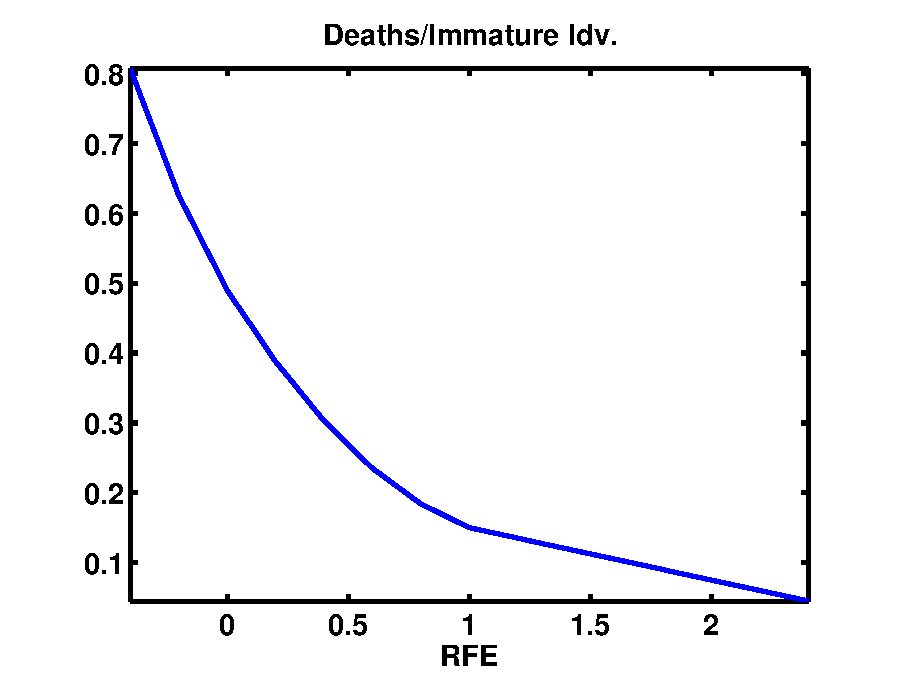
\includegraphics[width=0.9\textwidth]{mortImm}
\end{center}
\end{frame}

\begin{frame}
\begin{center}
\frametitle{\insertsection}
\begin{align}
  y_{\text{AF}}^{t+1} &= y_{\text{AF}}^t + y_{\text{YF}}^t - f_{\text{SF}}^ty_{\text{AF}}^t - f_{\text{MM}}^ty_{\text{AF}}^t \\
  y_{\text{NB}}^{t+1} &= f_{\text{C}}^ty_{\text{AF}}^t \\
  y_{\text{YF}}^{t+1} &= 0.5(y_{\text{NB}}^t - f_{\text{MI}}^ty_{\text{NB}}^t) - f_{\text{MM}}^ty_{\text{YF}}^t \\
  y_{\text{YM}}^{t+1} &= y_{\text{YM}}^t + y_{\text{NB}}^t - y_{\text{YF}}^{t+1} - f_{\text{SM}}^ty_{\text{YM}}^t - f_{\text{MM}}^ty_{\text{YM}}^t
\end{align}
\end{center}
\end{frame}

\section{General Characteristics}

\begin{frame}
\frametitle{Herd Dynamics Modeling}
\tableofcontents[currentsection]
\end{frame}


\begin{frame}
\begin{center}
\frametitle{\insertsection}
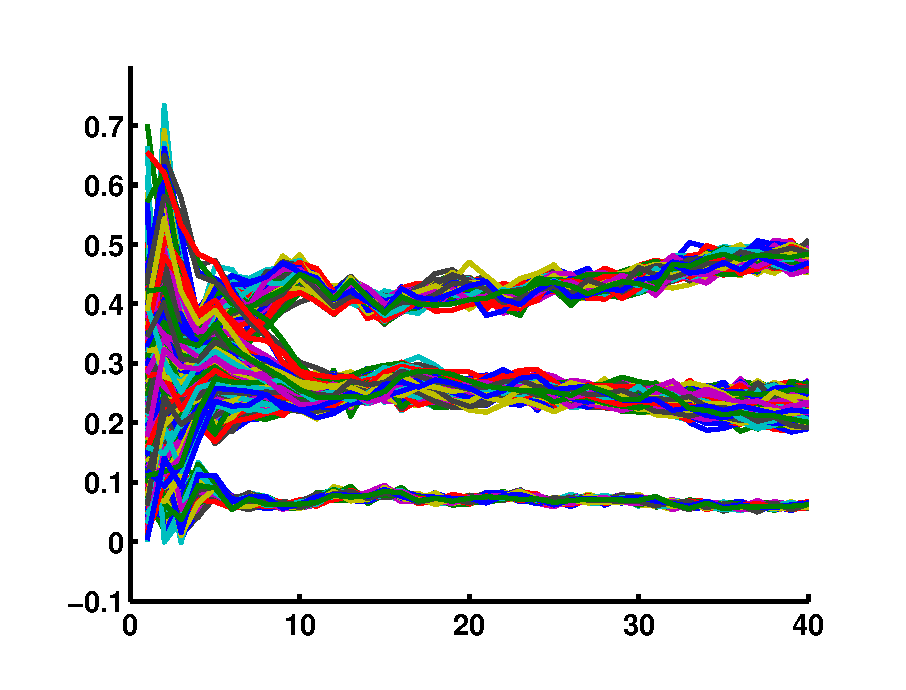
\includegraphics[width=0.9\textwidth]{ratios}
\end{center}
\end{frame}

\section{Data Assimilation}

\begin{frame}
\frametitle{Herd Dynamics Modeling}
\tableofcontents[currentsection]
\end{frame}

\begin{frame}
\begin{center}
\frametitle{\insertsection}
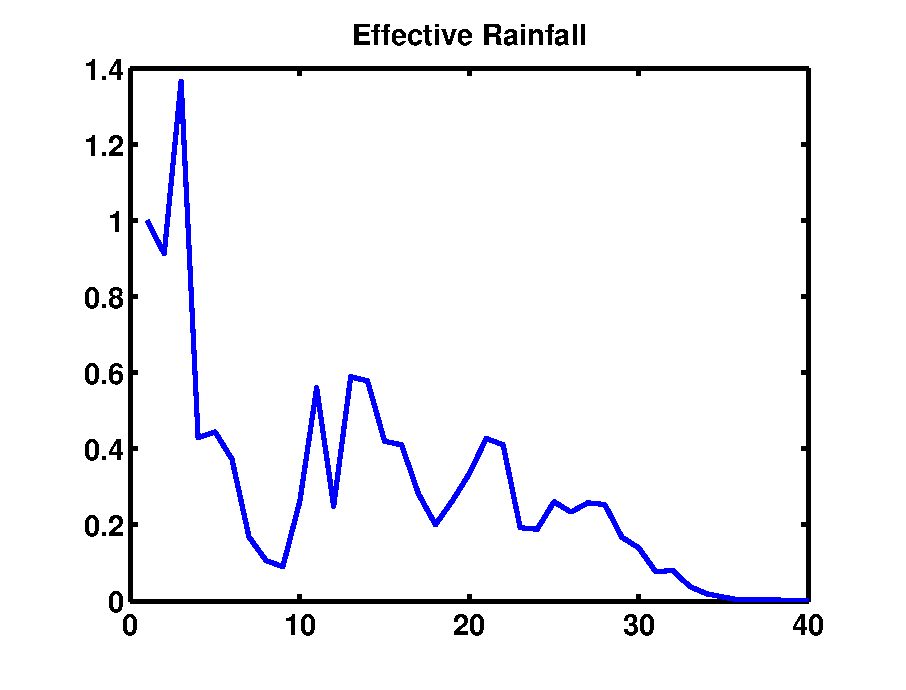
\includegraphics[width=0.9\textwidth]{forcing}
\end{center}
\end{frame}

\begin{frame}
\begin{center}
\frametitle{Synthetic Truth}
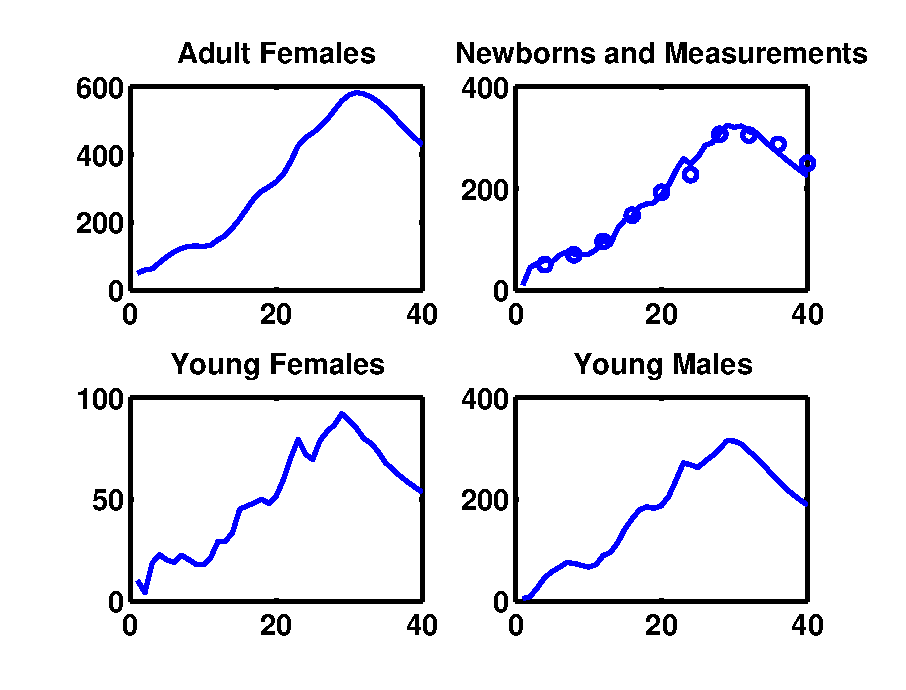
\includegraphics[width=1\textwidth]{truth}
\end{center}
\end{frame}

\subsection{Initial Conditions}

\begin{frame}
\begin{center}
\frametitle{Incorrect Initial Conditions}
\end{center}
\end{frame}

\begin{frame}
\begin{center}
\frametitle{Open Loop}
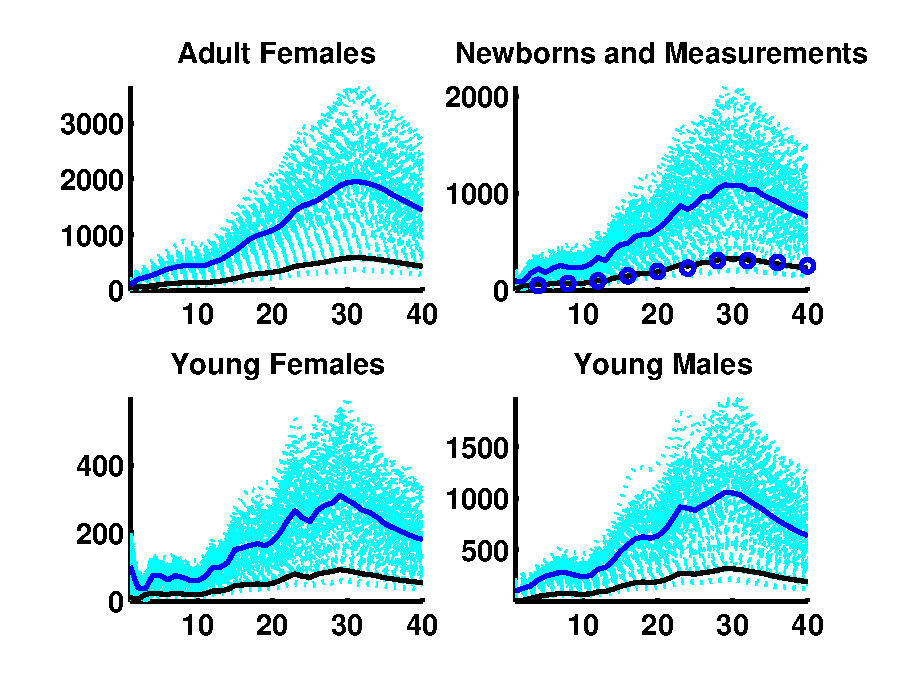
\includegraphics[width=1\textwidth]{openloop}
\end{center}
\end{frame}

\begin{frame}
\begin{center}
\frametitle{Ensemble Kalman Filter}
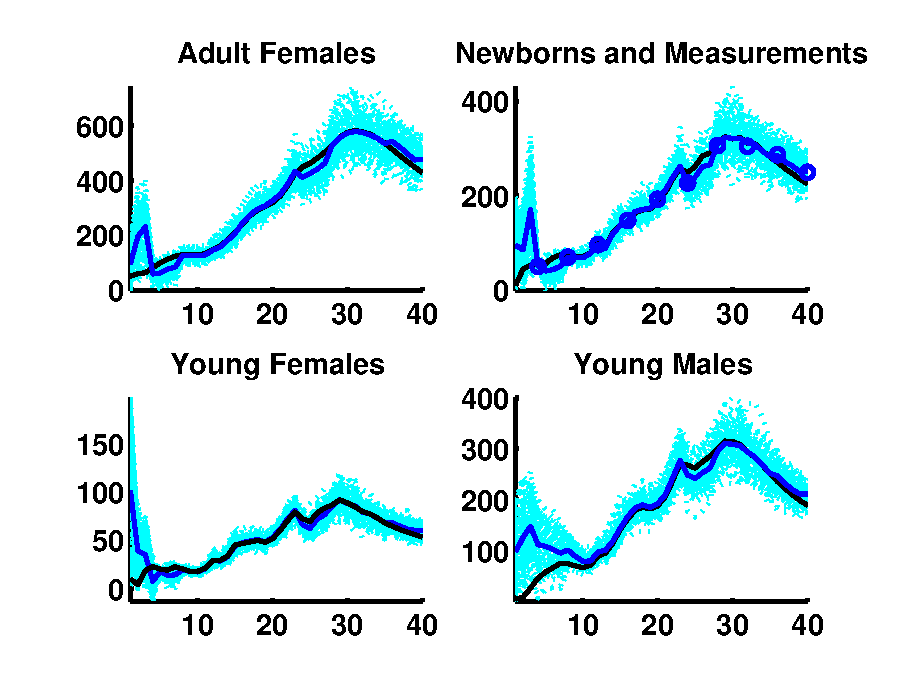
\includegraphics[width=1\textwidth]{filtered}
\end{center}
\end{frame}

\begin{frame}
\begin{center}
\frametitle{Ensemble Kalman Filter}
\begin{table}
\begin{tabular}{rrr}
& Bias & RMSE \\
\hline
Open loop & 441.2 & 565.2 \\
EnKF & 6.5 & 31.1
\end{tabular}
\caption{Skill of open loop vs. EnKF}
\end{table}
\end{center}
\end{frame}

\subsection{Ensemble Size}

\begin{frame}
\begin{center}
\frametitle{Ensemble Kalman Filter}
\begin{table}
\begin{tabular}{rrrr}
Ensemble members & 10 & 100 & 1000 \\
\hline
Bias & 10.5 & 6.5 & 6.5 \\
RMSE & 36.3 & 31.1 & 31.7
\end{tabular}
\caption{Skill for various ensemble sizes}
\end{table}
\end{center}
\end{frame}

\subsection{Model Error Variance}

%\bibliographystyle{plainnat}
%\bibliography{project}
\end{document}
